\documentclass{article}
\usepackage{geometry}
\usepackage{flafter}
\geometry{letterpaper, portrait, margin=1in}

\usepackage{hyperref}
\hypersetup{
    colorlinks=true,
    linkcolor=black,
    filecolor=magenta,
    urlcolor=blue,
}

\usepackage{graphicx}
\graphicspath{ {images/} }

\usepackage{tcolorbox}
\usepackage{textcomp}
\usepackage{gensymb}
\usepackage{indentfirst}
\usepackage{courier}

\newcommand{\ans}{$\rule{1.5cm}{0.15mm}$}

\title{RoboJackets Firmware Training Week 4 Lab Guide}
\author{Varun Madabushi, Joe Spall}
\date{\today\\v1.0}

\begin{document}
\maketitle{}
\setcounter{tocdepth}{2}
\tableofcontents
\pagebreak

%Everything below is for you to edit. Code above sets up the general formatting for the document

\section{Background}
    \subsection{Topics}
        The important topics being discussed this week in lab include communication protocols (specifically I2C), register mapping on datasheets, and sensors.
    \subsection{Premise}
        The lab premise is to use a training board with a mounted MPU-6050 sensor to detect \href{https://en.wikipedia.org/wiki/G-force}{g-force}. This \href{https://upload.wikimedia.org/wikipedia/en/f/f5/G-Force_poster.jpg}{g-force} can be used to determine what angle the training board is held. This angle will then be used to determine which 5 controllable LEDs will light up on-board, acting like a \href{https://en.wikipedia.org/wiki/Spirit_level}{bubble level indicator}.
    \subsection{Inertial Measurement}
        Inertial Measurement Units (IMUs) are a type of sensor that respond to changes in force applied to them. These consist of Accelerometers (which measure linear force) and Gyroscopes (which measure rotational velocity). These sensors are made up of Micro Electromechanical Systems (\href{https://en.wikipedia.org/wiki/Microelectromechanical_systems}{MEMS}) which are precisely tuned vibrating microstructures in the chip. Forces change the frequency of these vibrations, and that information is translated into electrical signals. These sensors are commonly used in robotics for measuring the pose (position and orientation) and motion of the robot in space.
        
        \begin{figure}[ht]
            \centering
            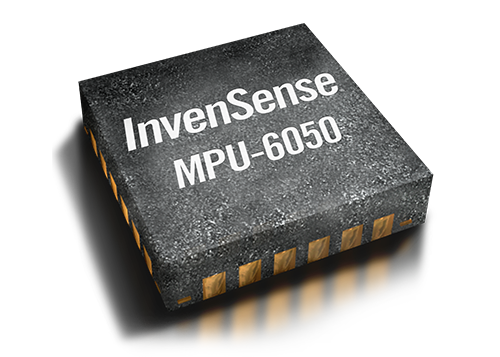
\includegraphics[width = 0.7\textwidth]{img/rp-mpu-6050.png}
            \caption{The MPU-6050 from TDK}
        \end{figure}
        For this lab we will be interfacing with the MPU-6050 Inertial Measurement Unit. Further information about the section can be found in Section \ref{readwrite}.
        
    \subsection{Simulation}
        If you are using a simulation instead of the hardware, do not worry.  The steps are exactly the same.  Go to the TinkerCad link and you will notice that the circuit has two Arduinos in it.  One is emulating the features of the IMU, and the other one is taking place of the actual Arduino that will be used to communicate with the IMU.
        
        \begin{figure}[ht]
            \centering
            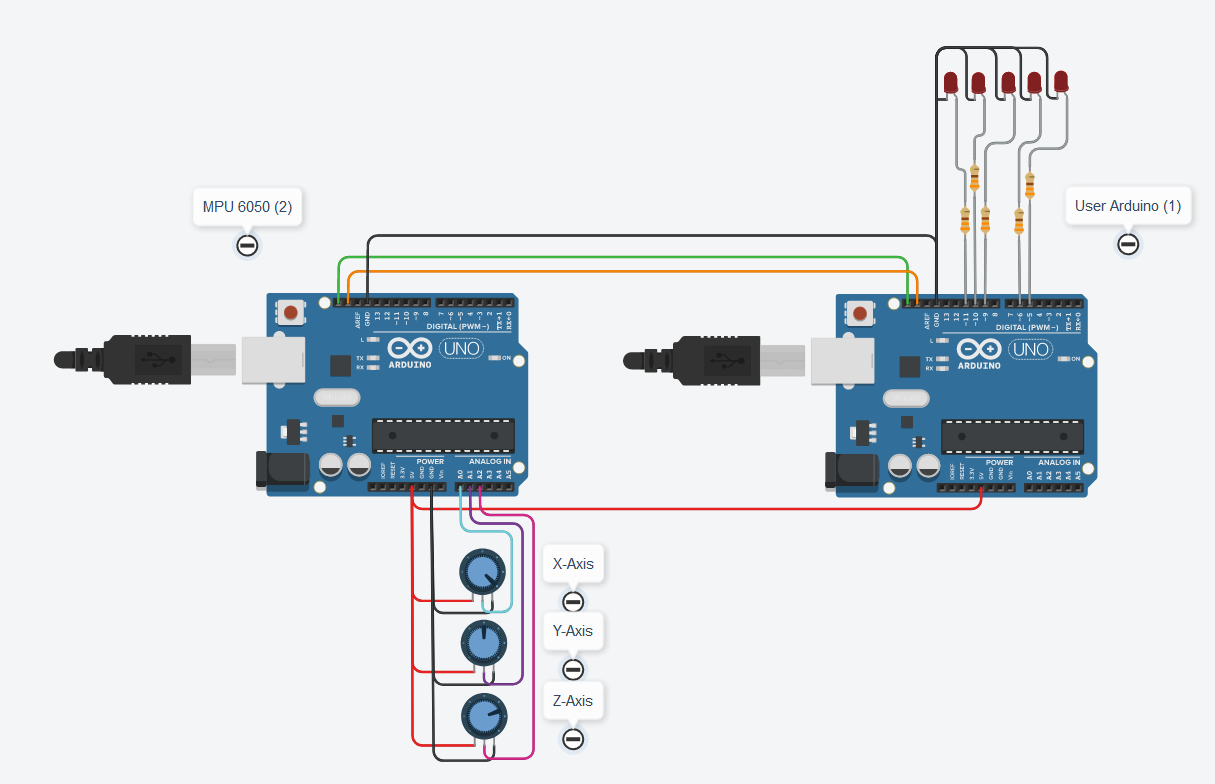
\includegraphics[width = 0.7\textwidth]{img/TinkerCadWires.PNG}
            \caption{The circuit window of TinkerCAD for this project}
        \end{figure}
        Since you can't tilt or move the IMU in the simulation, there are 3 knobs to represent the G-forces applied along each cardinal axis. Keeping the knob in the middle of the range represents 0 Gs, and the left-most or right-most rotations represent a negative or positive G-force at the max range. 
        
        \begin{figure}[ht]
            \centering
            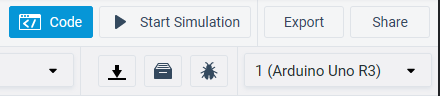
\includegraphics[width = 0.7\textwidth]{img/TinkerCadCode.PNG}
            \caption{The dropdown which you can use to select your target}
        \end{figure}
        
        The code for both Arduinos exists in the TinkerCAD code window. Arduino 1 is the target you should be writing code for, and Arduino 2 is running code to simulate the MPU-6050. You can switch between targets using the dropdown menu in the top-right corner of the screen. 
        \\ \\
        \textbf{NOTE: PLEASE DON'T EDIT THE MPU-6050 CODE TO REDUCE THE LIKELIHOOD OF ERRORS}
        
\section{Materials}
\begin{itemize}
	\item \href{https://www.autodesk.com/education/edu-software/overview}{AutoDesk Education Account}
	\item \href{https://www.tinkercad.com/things/16XnuyNUjCb}{TinkerCAD}
\end{itemize}

\section{Lab Objectives}
    \subsection{Task 1 - Get the IMU to turn on}

        \begin{enumerate}
            \item Set the IMU to 'Awake' by writing 0 to \texttt{PWR\_MGMT\_1}
            \begin{itemize}
                \item The register names for a few relevant registers have been predefined in the code template. Please take a moment to look through these at the top of the code file. They can be accessed directly by name.
                \item Page 41-42 of the MPU-6050 \href{https://cdn.sparkfun.com/datasheets/Sensors/Accelerometers/RM-MPU-6000A.pdf}{datasheet} shows the various fields of this register.
                \item Writing 0 to this register sets all bits such that the device is not reset, the sleep mode is disabled, the chip does not cycle on-off, the temperature sensor is enabled, and the internal oscillator is used.
                \item A refresher on reading and writing from external devices with I2C can be found in Section \ref{readwrite}.
            \end{itemize}
            \item Run a "Who Am I" test to ensure communication.
            \begin{itemize}
                \item A "Who Am I" test asks the chip to return a known value so we can ensure data is transferring smoothly.
                \item Read from the \texttt{WHO\_AM\_I} register and use Arduino's \texttt{Serial.print()} to print the result to the console. This should return the value specified in the register map. 
            \end{itemize}
        \end{enumerate}

    \subsection{Task 2 - Read raw data}\label{Sec2}
        \begin{enumerate}
            \item We would like to read the X, Y, and Z accelerations from the IMU, so we must request these values from the sensor with \texttt{Wire.requestFrom()}.
            \begin{itemize}
                \item Each acceleration value is represented by 16 bits spread across 2 8-bit (1 byte) registers.
                \item We want to read from 6 registers starting from \texttt{ACCEL\_XOUT\_H} (\texttt{0x38}).
                \item Refer to Page 30 of the MPU-6050 datasheet for more information.
            \end{itemize}
            \item Now, receive the individual bytes and reconstruct them into sensor readings.
            \begin{itemize}
                \item The High byte (e.g. \texttt{ACCEL\_XOUT\_H}) corresponds to the first 8 bits, while the low byte (e.g. \texttt{ACCEL\_XOUT\_L}) corresponds to the last 8 bits.
                \item These must be combined into a 16-bit data type (such as \texttt{int16\_t}).
                \item Shift the high byte over by 8 bits and bitwise-OR it with the low byte.
            \end{itemize}
            \item Lastly, we must convert the \texttt{int16\_t} values into decimal accelerations in Gs.
            \begin{itemize}
                \item Data usually comes in units of least significant bits (LSBs), which are divisions of the Full-Scale Range into $2^{BIT\_DEPTH}$ number of divisions.
                \item The \texttt{AFS\_SEL} register changes the Full-Scale range of the sensor and thus sets the conversion factor between LSBs and Gs.
            \end{itemize}
            \item Print the resulting G-Force values to the console to make sure they are reasonable.
            \begin{itemize}
                \item If you have the board, place it stationary and flat on the table, \texttt{x\_g} and \texttt{y\_g} should be close to 0, and \texttt{z\_g} should be close to 1.
                \item If you do not have a board, adjust the potentiometer to make sure the range is what you expect.
            \end{itemize}
        \end{enumerate}
        
    \subsection{Task 3 - Use acceleration data to light up LEDs}
        \begin{enumerate}
            \item Instantiate a struct to hold the acceleration vector.
            \begin{itemize}
                \item Construct an instance of the vector struct by creating a new \texttt{tb::Vector3D}. 
                \item Assign each of the fields \texttt{x\_g, y\_g, z\_g}  of your new \texttt{Vector3D} variable using the values calculated in Section \ref{Sec2} step 3. 
            \end{itemize}
            \item Light up LEDs corresponding to value in the struct.
            \begin{itemize}
                \item A method, \texttt{setBubbleIndicator(tb::Vector3D vector)}, is also provided for you.
                \item Pass the \texttt{tb::Vector3D} struct into this method, and your LEDs should light up corresponding to the angle. 
                \item NOTE: If you are using the simulator, this step will only work if you set the y-axis acceleration to 0 and set the z axis acceleration to 1G (about half the positive range).
            \end{itemize}
        \end{enumerate}
    

\section{Relevant Information}
    \subsection{MPU-6050} \label{readwrite}
        The MPU-6050 is an Inertial Measurement Unit (\href{https://en.wikipedia.org/wiki/Inertial_measurement_unit}{IMU}) which is mounted to the training board by means of a breakout board (the smaller PCB).  
        In order to control it, first familiarize yourself with the register map found \href{https://cdn.sparkfun.com/datasheets/Sensors/Accelerometers/RM-MPU-6000A.pdf}{here}.
        
        As per the datasheet, communicating with this involves interacting with the internal read/write pointer of the microcontroller. \\
        
        \noindent If you wish to write to a particular register, the following steps must be taken:
        \begin{enumerate}
            \item Begin a transmission (\texttt{Wire.beginTransmission(DEV\_ADDR)}).
            \item Send the address of the register you wish to write to (\texttt{Wire.write(REG\_ADDR)}).
            \item Send the value you wish to write to the register (\texttt{Wire.write(VALUE})).
            \item End the transmission (\texttt{Wire.endTransmission()}).
        \end{enumerate}
        \noindent A similar process can be followed for reading from registers:
        \begin{enumerate}
            \item Begin a transmission (\texttt{Wire.beginTransmission(DEV\_ADDR)}).
            \item Send the address of the register you wish to start reading from (\texttt{Wire.write(REG\_ADDR)}).
            \item End the transmission (\texttt{Wire.endTransmission()}).
            \item Request a number of bytes you want to receive (\texttt{Wire.requestFrom(DEV\_ADDR, BYTES, true)}).
            \item Read in the bytes, repeating for the number of bytes to be read (\texttt{Wire.read()})
        \end{enumerate}
    \subsection{Important MPU-6050 Registers}\label{registers}
        The particular registers we use in this lab are the following: 
        \begin{itemize}
            \item \texttt{PWR\_MGMT\_1} - Turns on device
            \item \texttt{WHO\_AM\_I} - Identifies device
            \item \texttt{ACCEL\_XOUT\_H} - Accelerometer X, high 8 bits 
            \item \texttt{ACCEL\_XOUT\_L} - Accelerometer X, low 8 bits 
            \item \texttt{ACCEL\_YOUT\_H} - Accelerometer Y, high 8 bits
            \item \texttt{ACCEL\_YOUT\_L} - Accelerometer Y, low 8 bits 
            \item \texttt{ACCEL\_ZOUT\_H} - Accelerometer Z, high 8 bits
            \item \texttt{ACCEL\_ZOUT\_L} - Accelerometer Z, low 8 bits 
            \item \texttt{ACCEL\_CONFIG} - contains scaling between bits and g-force
        \end{itemize}
        
        A good practice for readability is to reference these registers by name in the code. To do this, first fill out \texttt{\#define} statements which will represent the hexadecimal values of the registers as readable words. For example, the statement \texttt{\#define PWR\_MGMT\_1 0x6b} gives the text \texttt{PWR\_MGMT\_1} a value of \texttt{0x6b} in the code.  
        
    \subsection{\texttt{Wire} Library}
        The library we will be using for I2C communication is the \texttt{Wire} Library. You can refer to the reference page \href{https://www.arduino.cc/en/reference/wire}{here} for understanding the necessary functions along with examples.
        
        \begin{figure}[ht]
            \centering
            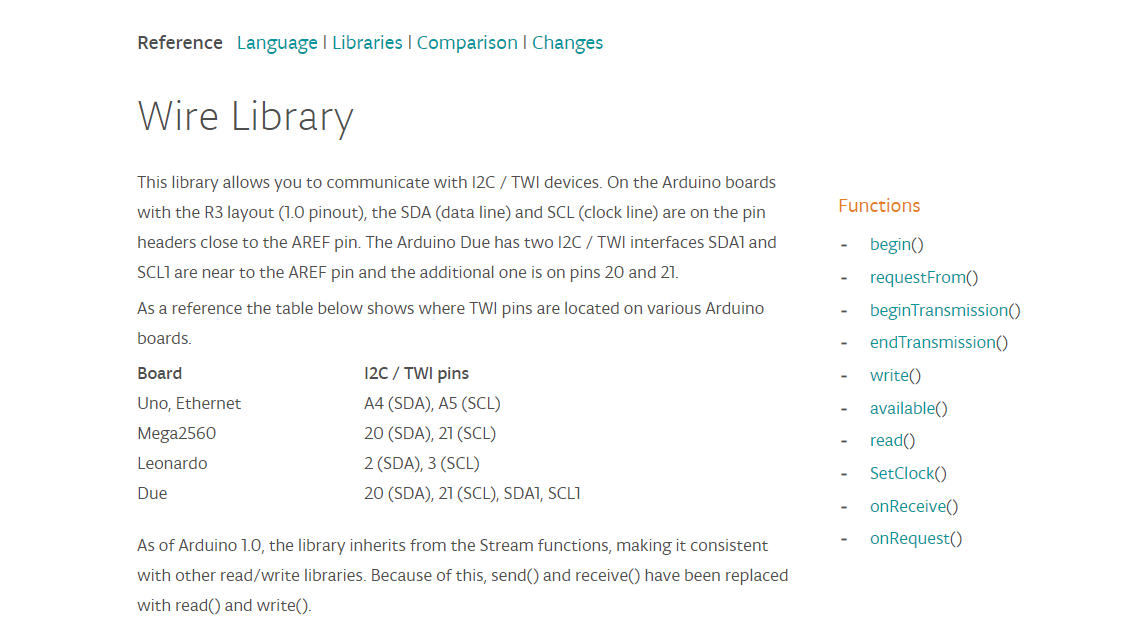
\includegraphics[width = 1.0\textwidth]{img/WireLibrary.PNG}
            \caption{\texttt{Wire} Library on the Arduino website}
        \end{figure}
        
\section{Troubleshooting}
    \subsection{Solutions}
    We have included the solutions below if you do not complete the lab during the session or if you want to verify your answer. If you need help during the lab ask an instructor!
\begin{itemize}
    \item \href{https://www.tinkercad.com/things/lFJojnkgwTw}{TinkerCAD Solution}
    \end{itemize}
    
    \section{Egg}
    There is a virtual egg in this document. If you find it, contact the authors of this document with proof of what you think the virtual egg is and you will receive one (1) real egg in return. 
\end{document}
